% SETUP DOCUMENTO %
\documentclass[onecolumn]{article}
\usepackage[italian]{babel}

\usepackage{tgschola}
\linespread{1.25}
\usepackage[fontsize=12pt]{scrextend}
\usepackage[a4paper,top=2.5cm,bottom=2.5cm,left=3cm,right=3cm,marginparwidth=1.75cm,footskip=1.5cm,heightrounded]{geometry}

\usepackage{xcolor}
\usepackage{amsmath}
\usepackage[bottom]{footmisc}

% IMMAGINI %
\usepackage{subfig}
\usepackage{graphicx}
\usepackage{float}
\graphicspath{ {./images/} }

% TABELLE %
\usepackage{adjustbox}
\usepackage{booktabs}

% STILE LINK ESTERNI %
\definecolor{linkColor}{RGB}{2,11,120}
\usepackage[colorlinks=true, allcolors=linkColor]{hyperref}
\newcommand\anchor[2]{%
  \href{#2}{#1}\footnote{\url{#2}}%
}

% STILE BLOCCHI DI CODICE %
\definecolor{bgTitleRed}{RGB}{85,45,50}
\usepackage[T1]{fontenc}
\usepackage[ttdefault=true]{AnonymousPro}
\usepackage{listings}
\usepackage{minted}
\usepackage{tcolorbox}
\tcbuselibrary{listings, breakable, minted, skins}
\tcbset{listing engine=minted}

\newtcblisting{bashCode}[2][]{
    breakable,
    listing only, #1 ,title=#2,
    minted language=bash,
    minted style=vs,
    coltitle=white,
    colbacktitle=bgTitleRed,
    toptitle=3mm, bottomtitle=2.5mm,
    top=2mm, bottom=3mm,
    fonttitle=\ttfamily,
    enhanced, frame hidden, 
    minted options={fontfamily=AnonymousPro, 
    tabsize=4, breaklines, autogobble, linenos=false}}

\setminted[python]{fontfamily=AnonymousPro, fontsize=\footnotesize, breaksymbol=.}

% INTESTAZIONE %
\title{Relazione Laboratorio Algoritmi\\\textit{Esercizio B}}
\author{Alberto Del Buono Paolini}
\date{Ottobre 2023}

\begin{document}
\begin{onecolumn}
	\vspace*{-6em}
	{\let\newpage\relax\maketitle}
	\vspace*{-2em}
	\tableofcontents
\end{onecolumn}
\vspace{1cm}
\pagebreak

% CONTENUTO %
\section{Descrizione del problema}

\subsection{Introduzione}
Questa relazione vuole analizzare e commentare il calcolo delle statistiche d'ordine dinamiche \textit{OS-Select} e \textit{OS-Rank}, mettendo a confronto le seguenti strutture dati: 
\begin{enumerate}
	\setlength\itemsep{-0.25em}
	\item Lista ordinata collegata con puntatori
	\item Albero binario di ricerca senza attributo \textit{size}
	\item Albero rosso-nero con attributo \textit{size}
\end{enumerate}

L'obiettivo è valutare le prestazioni e le caratteristiche di ciascuna implementazione attraverso test ed esperimenti pratici, confrontandole con le evidenze teoriche descritte nella prossima sezione.

\subsection{Caratteristiche teoriche}

Per prima cosa dobbiamo descrivere la natura di queste tre strutture dati e delle statistiche d'ordine dinamiche che andremo ad analizzare. Esamineremo quindi nei vari casi le complessità computazionali di:

\begin{enumerate}
	\setlength\itemsep{-0.25em}
	\item \textit{OS-Select(k)}: è un'operazione che trova l'elemento con rango $k$ in un insieme di dati, cioè restituisce il $k$-esimo elemento più piccolo dell'insieme di dati.
	\item \textit{OS-Rank(x)}: è un'operazione che calcola il rango di un elemento $x$ all'interno di un insieme di dati, cioè restituisce il numero di elementi nell'insieme che sono inferiori o uguali a $x$.
\end{enumerate}

\subsubsection{Lista collegata ordinata}

Questa è una struttura composta da nodi che hanno attributi \textit{value} (il valore del dato contenuto nel nodo) e \textit{next} (un puntatore al nodo successivo della lista oppure vuoto). Per attraversare completamente una lista collegata con puntatori bisogna quindi partire dal primo nodo (chiamato solitamente \textit{head}) e spostarsi sui nodi successivi tramite il puntatore \textit{next}, fino a che non è vuoto, a significare la fine della lista. Inoltre è una struttura ordinata: ogni nodo viene inserito nella lista in base al valore del suo dato (con ordine ascendente o discendente). Supponiamo di essere nel caso di ordine ascendente, come mostrato in \hyperref[fig:lista]{figura 1}.

\begin{figure}
	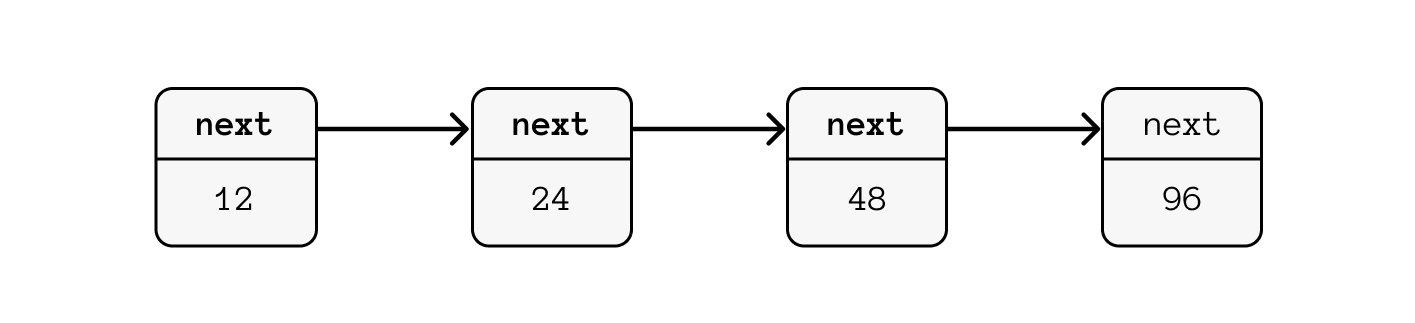
\includegraphics[width=\linewidth]{lista.png}
	\caption{Lista collegata con puntatori}
	\label{fig:lista}
\end{figure}

\textbf{OS-Select}: questa operazione richiede di scorrere la lista dall'inizio, contando gli elementi fino a raggiungere il $k$-esimo. Questo significa che il tempo necessario per trovare questo elemento cresce linearmente con $k$ e, nel caso peggiore, bisognerà quindi scorrere tutta la lista lunga $n$. La complessità di OS-Select è quindi $O(k)$ e $\Theta(n)$ nel caso peggiore. \vspace{0.5em}

\textbf{OS-Rank}: Per determinare il rango di un elemento x bisogna scorrere la lista contando quante chiavi sono inferiori a $x$, perciò le complessità sono uguali a OS-Select. La lista collegata ordinata non è molto efficiente per il calcolo delle due statistiche d'ordine, specialmente quando si cerca un $k$ o un $x$ grande. 

\subsubsection{Albero binario di ricerca}

Un albero binario di ricerca è una struttura dati gerarchica composta da nodi collegati tra loro. Ogni nodo ha attributi per al massimo due figli, uno a sinistra (\textit{left}) e uno a destra (\textit{right}), e un valore (\textit{value}) che soddisfi le seguenti proprietà:

\begin{enumerate}
	\setlength\itemsep{-0.25em}
	\item I valori nei nodi del sottoalbero sinistro sono inferiori o uguali al valore nel nodo padre.
	\item I valori nei nodi del sottoalbero destro sono superiori al valore nel nodo padre.
\end{enumerate}

Quindi per qualsiasi nodo nell'ABR (illustrato in \hyperref[fig:alberi]{figura 2a}), tutti i nodi nei sottoalberi a sinistra contengono valori inferiori o uguali, e tutti i nodi nei sottoalberi a destra contengono valori superiori; questo aiuta la complessità del calcolo delle statistiche d'ordine. \vspace{1em}

\textbf{OS-Select}: Questo metodo attraversa un singolo percorso nell'albero per trovare il $k$-esimo elemento e la complessità è $O(h)$, dove $h$ è l'altezza dell'albero. Il tempo di esecuzione dipende dall'altezza dell'albero e dalla struttura specifica dell'albero. Se l'albero è bilanciato, l'altezza è $\Theta(\log n)$, garantendo una complessità di $O(\log n)$ nel caso peggiore. \vspace{0.5em}

\textbf{OS-Rank}: anche OS-Rank richiede un percorso nell'albero fino a un elemento specifico $x$ e ha una complessità temporale di $O(h)$. Sarebbe necessaria la costante riequilibratura dell'albero per mantenere la complessità $O(\log n)$. Tuttavia, se l'albero è sbilanciato con un unico ramo, la complessità può arrivare fino a $\Theta(n)$, ugualmente ad OS-Select.

\begin{figure}
	\centering
	\subfloat[Albero binario di ricerca]{{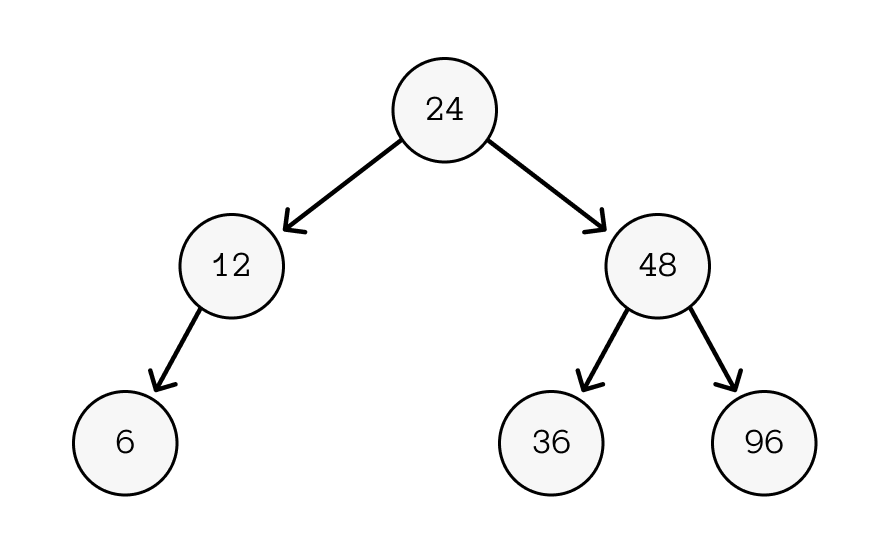
\includegraphics[width=\linewidth/2-1.5em]{abr} }}
	\qquad
	\subfloat[Albero rosso-nero aumentato]{{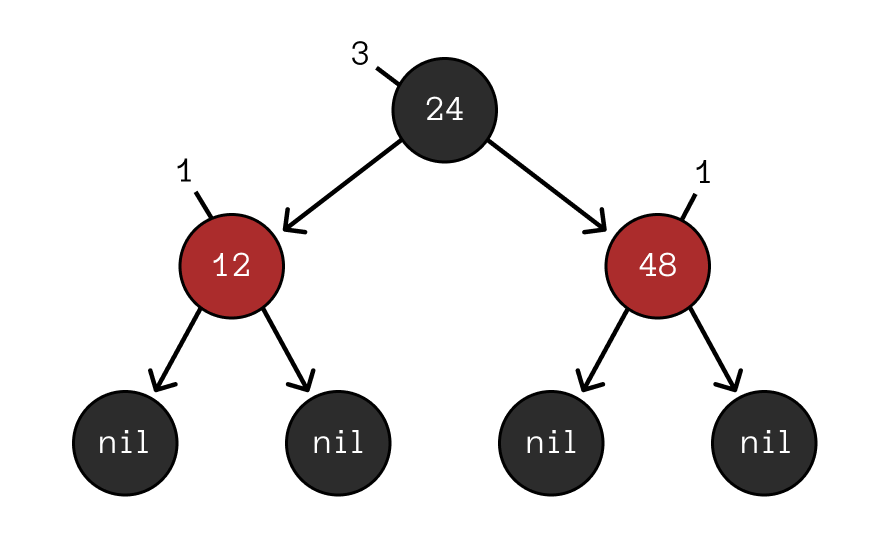
\includegraphics[width=\linewidth/2-1.5em]{arn} }}
	\caption{Illustrazioni alberi}
	\label{fig:alberi}
\end{figure}

\subsubsection{Albero rosso-nero aumentato con attributo \textit{size}}

Gli alberi rosso-neri aumentati sono una variante dei tradizionali alberi rosso-neri. Le proprietà di un albero rosso-nero sono estese da quelle di un albero binario di ricerca con un etichetta per ogni nodo come \textit{rosso} o \textit{nero} nell'attributo \textit{color}, seguendo le seguenti regole per garantire che l'albero sia bilanciato:

\begin{enumerate}
	\setlength\itemsep{-0.25em}
	\item Un nodo è o rosso o nero.
	\item La radice dell'albero è nera.
	\item Non possono esistere due nodi rossi consecutivi lungo qualsiasi cammino dall'alto verso il basso.
\end{enumerate}

Gli ARN aumentati (in \hyperref[fig:alberi]{figura 2b}) includono una modifica aggiuntiva: l'attributo \textit{size} in ciascun nodo dell'albero. Questo attributo tiene traccia del numero di nodi nel sottoalbero con radice in quel nodo (include anche il nodo stesso) e velocizza in media il calcolo del rango di un elemento all'interno dell'albero. \vspace{1em}

\textbf{OS-Select}: l'operazione di OS-Select è molto efficiente grazie all'attributo \textit{size}, possiamo trovare il $k$-esimo elemento sempre in $O(h)$ e $\Theta(\log n)$ nel caso peggiore. \vspace{0.5em}

\textbf{OS-Rank}: Anche l'operazione di OS-Rank ha una complessità di $O(h)$ e di $\Theta(\log n)$ nel caso peggiore. \vspace{1em}

In generale, l'implementazione con l'albero rosso-nero aumentato con l'attributo \textit{size} eccelle nel calcolo di entrambe le statistiche d'ordine, offrendo prestazioni notevolmente migliori rispetto agli ABR non bilanciati, essendo bilanciati ad ogni nuovo inserimento. Le complessità per le varie strutture sono riassunte in \hyperref[tab:complessita]{tabella 1}.

\begin{table}[t]
	\centering
	\begin{tabular}{|c|c|c|c|}
		\hline
		& Lista ordinata & \hspace*{2em}ABR\hspace*{2em} & ARN aumentato \\
		\hline
		\textbf{OS-Select} & $O(k)$         & $O(\log n)$                   & $O(\log n)$   \\
		\hline
		\textbf{OS-Rank}   & $O(n)$         & $O(\log n)$                   & $O(\log n)$   \\
		\hline
	\end{tabular}
	\caption{Complessità delle statistiche d'ordine}
	\label{tab:complessita}
\end{table}

\section{Descrizione degli esperimenti}
\subsection{Piattaforma di esecuzione}

Per sviluppare il codice ed eseguire tutti i test, ottenendo le tabelle e i grafici riportati in questo documento, è stata utilizzata un'istanza di \anchor{Gitpod}{https://www.gitpod.io/} con le seguenti specifiche:
\begin{bashCode}{Output neofetch}
	OS: Ubuntu 22.04.3 LTS x86_64 
	Host: Google Compute Engine 
	Kernel: 6.1.54-060154-generic 
	CPU: AMD EPYC 7B13 (16 cores) @ 2.449GHz 
	Memory: 64297MiB
\end{bashCode}

\subsection{Dimensione e popolazione delle strutture}

E' fondamentale eseguire i test su diverse dimensioni delle strutture dati per valutare come le prestazioni variano con l'aumento del numero di elementi. Andremo a testare le prestazioni su insiemi di dati di dimensioni:
\begin{enumerate}
	\setlength\itemsep{-0.25em}
	\item 10 - 1000 (\textit{Dimensioni ridotte})
	\item 1000 - 10000 (\textit{Dimensioni medie})
	\item 10000 - 20000 (\textit{Dimensioni elevate})
\end{enumerate}

Per il primo intervallo i test verranno eseguiti su ogni dimensione tra 10 e 1000 con passo \textbf{10} (10, 20, 30, ...). Per il secondo intervallo le dimensioni sono scelte in maniera più sparsa con passo di \textbf{100}. Per il terzo intervallo invece sono eseguite con passo di \textbf{500} a causa del maggior tempo di esecuzione. \vspace{1em}

Ogni struttura dati, prima dei test sulle statistiche d'ordine, viene popolata in modo casuale con uno dei seguenti tipi di dato:
\begin{enumerate}
	\setlength\itemsep{-0.25em}
	\item \textit{Valori interi} random compresi tra 1 e 5000
	\item \textit{Valori float} random compresi tra 1 e 1000
\end{enumerate}

\subsection{Strategia di iterazione e misurazione}

Per ogni struttura dati e per ogni statistica d'ordine dinamica verranno eseguiti i test un certo numero di iterazioni (consideriamo \textbf{1000} come numero sufficiente) per ogni dimensione specificata. Per ognuna di queste iterazioni, le due operazioni saranno svolte in modo casuale sugli elementi della struttura dati, andando a simulare uno scenario realistico di utilizzo delle statistiche d'ordine. 

Raccoglieremo poi la mediana dei tempi di esecuzione per ogni dimensione, producendo i rispettivi grafici. Questo metodo riduce l'impatto di variazioni casuali e fornisce risultati più stabili.

Per ogni misurazione saranno proposti due grafici, uno che usa il tempo effettivo di esecuzione delle istruzioni e un altro che utilizza un tempo relativo alla dimensione dell'insieme di dati (utile per visualizzare la complessità computazionale nei vari casi), calcolati come segue:
\begin{enumerate}
	\setlength\itemsep{-0.25em}
	\item \textit{Tempo effettivo}: \verb|end_time - start_time|
	\item \textit{Tempo relativo}: \verb|(end_time - start_time) / size|
\end{enumerate}

Tutte le misurazioni dei tempi sono effettuate usando la libreria \verb|timeit| che ci fornisce risultati di esecuzione accurati. 

I test completi su tutte le strutture sono eseguiti nel file \verb|main.py|, insieme al salvataggio dei relativi grafici e tabelle.

\newpage
\section{Documentazione del codice}

La struttura delle classi è osservabile nel diagramma UML in \hyperref[fig:classi]{figura 3}; segue anche una breve descrizione di ogni attributo e metodo implementato per le tre strutture dati. Tutti gli attributi e i metodi sono corredati di annotazioni di tipo nel codice (validate con \verb|mypy|). La cronologia completa dello sviluppo è disponibile su una repository Github pubblica reperibile tramite \anchor{questo link}{https://github.com/albbus-stack/lab-alg}. 

\begin{figure}[h!]
	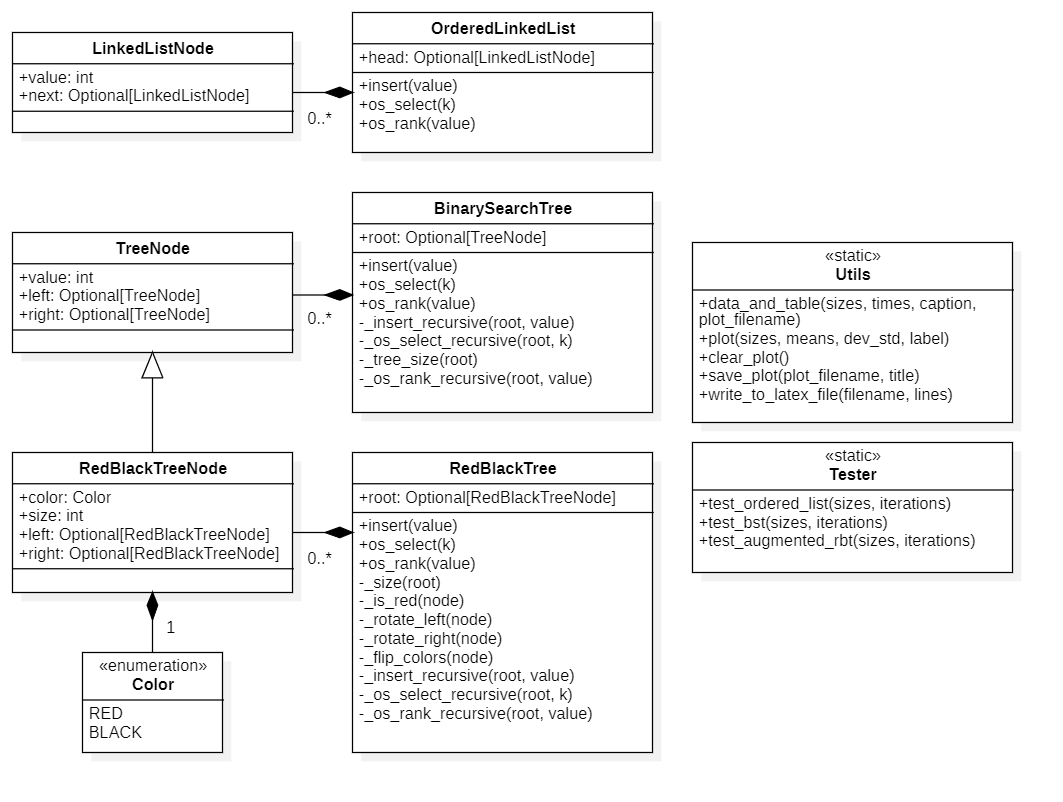
\includegraphics[width=\linewidth]{classi.png}
	\caption{Diagramma UML delle classi}
	\label{fig:classi}
\end{figure}

\subsection{Lista collegata ordinata}
\texttt{\textbf{LinkedListNode}}
\begin{itemize}
	\setlength\itemsep{0em}
	\item \verb|value|: il valore memorizzato nel nodo
	\item \verb|next|: il riferimento al nodo successivo
\end{itemize}

{\setlength{\parindent}{0em} \texttt{\textbf{OrderedLinkedList}}}
\begin{itemize}
	\setlength\itemsep{0em}
	\item \verb|head|: il riferimento al primo nodo nella lista (di tipo \texttt{LinkedListNode})
	\item \verb|insert(value)|: inserisce un nuovo nodo nella lista con il valore specificato 
	\item \verb|os_select(k)|: restituisce il valore dell'elemento con rango $k$ nella lista
	\item \verb|os_rank(value)|: restituisce il rango dell'elemento con valore specificato nella lista
\end{itemize}

\subsection{Albero binario di ricerca}
\texttt{\textbf{TreeNode}}
\begin{itemize}
	\setlength\itemsep{0em}
	\item \verb|value|: il valore memorizzato nel nodo
	\item \verb|left|: il riferimento al figlio sinistro del nodo
	\item \verb|right|: il riferimento al figlio destro del nodo
\end{itemize}

{\setlength{\parindent}{0em} \texttt{\textbf{BinarySearchTree}}}
\begin{itemize}
	\setlength\itemsep{0em}
	\item \verb|root|: il riferimento alla radice dell'albero (di tipo \texttt{TreeNode})
	\item \verb|insert(value)|: inserisce un nuovo nodo con il valore specificato nell'ABR, usa il metodo privato ricorsivo \newline \verb|_insert_recursive(root, value)| a partire dalla radice.
	\item \verb|_tree_size(root)|: calcola la dimensione del sottoalbero radicato in un nodo specifico ricorsivamente
	\item \verb|os_select(k)|: restituisce il valore dell'elemento con rango $k$ usando il metodo privato ricorsivo \verb|_os_select_recursive(root, k)| che naviga l'albero a seconda della dimensione dei sottoalberi 
	\item \verb|os_rank(value)|: restituisce il rango dell'elemento con valore specificato  usando il metodo privato \verb|_os_rank_recursive(root, value)| che cerca ricorsivamente \textit{value} nell'albero e restituisce la dimensione del suo sottoalbero
\end{itemize}

\subsection{Albero rosso-nero aumentato con attributo \textit{size}}
\texttt{\textbf{RedBlackTreeNode}}
\begin{itemize}
	\setlength\itemsep{0em}
	\item \verb|color|: il colore del nodo (di tipo \texttt{Color}: \texttt{RED} o \texttt{BLACK})
	\item \verb|size|: il numero di nodi nel sottoalbero radicato in questo nodo
	\item \verb|left|: il riferimento al figlio sinistro del nodo
	\item \verb|right|: il riferimento al figlio destro del nodo
	\item \verb|value|: il valore memorizzato nel nodo (ereditato dalla classe \texttt{TreeNode})
\end{itemize}

\newpage
{\setlength{\parindent}{0em} \texttt{\textbf{AugmentedRedBlackTree}}}
\begin{itemize}
	\setlength\itemsep{0em}
	\item \verb|root|: il riferimento alla radice dell'ARN aumentato (di tipo \texttt{RedBlackTreeNode})
	\item \verb|insert(value)|: inserisce un nuovo nodo con un certo valore nell'albero rosso-nero aumentato; usa il metodo ricorsivo \texttt{\_insert\_recursive(root, value)} che, dopo aver inserito il valore, bilancia l'albero
	\item \verb|os_select(k)|: restituisce il valore dell'elemento con rango $k$ nell'albero rosso-nero aumentato, la sua implementazione è uguale a quella dell'albero binario di ricerca, a parte per il metodo \texttt{\_size(node)}
	\item \verb|os_rank(value)|: restituisce il rango dell'elemento col valore specificato e anche la sua implementazione è la stessa degli ABR, a parte per il metodo \texttt{\_size(node)}
	\item \verb|_size(node)|: ritorna l'attributo \textit{size} oppure 0 se il nodo è \texttt{None}
	\item \verb|_is_red(node)|: ritorna \texttt{True} se il nodo ha colore rosso oppure \texttt{False} se il nodo è nero o \texttt{None}
	\item \verb|_rotate_left(node)|: esegue una rotazione sinistra del sottoalbero rosso-nero con radice nel nodo
	\item \verb|_rotate_rigth(node)|: esegue una rotazione destra del sottoalbero rosso-nero con radice nel nodo
	\item \verb|_flip_colors(node)|: inverte i colori di un nodo e dei suoi due figli nell'ARN
\end{itemize}

\subsection{Classi statiche \texttt{Tester} e \texttt{Utils}}

Queste classi contengono tutti metodi statici che sono stati raggruppati semanticamente in esse.
\vspace{0.75em}
\newline
\texttt{\textbf{Tester}}
\begin{itemize}
	\setlength\itemsep{0em}
	\item \verb|test_ordered_list(sizes, iterations, ...)|: esegue test e raccolta dati per la lista collegata ordinata
	\item \verb|test_bst(sizes, iterations, ...)|: esegue test e raccolta dati per l'albero binario di ricerca
	\item \verb|test_augmented_rbt(sizes, iterations, ...)|: esegue test e raccolta dati per l'albero rosso-nero aumentato con attributo \textit{size}
\end{itemize}

\newpage
{\setlength{\parindent}{0em} \texttt{\textbf{Utils}}}
\begin{itemize}
	\setlength\itemsep{0em}
	\item \verb|table_and_medians(sizes, times, caption, plot_filename)|: genera e restituisce mediane ed errori insieme per la creazione dei grafici e delle tabelle \LaTeX\ o \verb|.csv|
	\item \verb|plot(sizes, medians, label)|: crea un grafico con le mediane e dimensioni in ingresso
	\item \verb|clear_plot()|: cancella il grafico corrente
	\item \verb|save_plot(plot_filename, title)|: salva il grafico corrente in un \verb|.png| con un titolo specificato
	\item \verb|write_to_latex_file(filename, df_and_captions)|: scrive le linee del \verb|DataFrame| in una tabella \TeX\ e \verb|.csv| con il nome specificato.
\end{itemize}

\newpage
\section{Analisi dei risultati sperimentali}

In questa sezione verranno analizzati risultati sperimentali, discutendo le discrepanze tra le prestazioni attese e quelle effettivamente osservate, se presenti, e verranno offerte interpretazioni basate esclusivamente sui dati raccolti. Tutti i grafici presenti in questa sezione hanno illustrata la mediana per le 1000 iterazioni relative ad una dimensione di test come descritto precedentemente. I dati illustrati sono riportati nelle tabelle dell'appendice, corredati anche delle deviazioni dal minimo e dal massimo (errori) rispetto alla mediana, a cui viene fatto riferimento nel testo.

\subsection{Dimensioni ridotte}

\begin{figure}[H]
	\subfloat[Tempi assoluti (interi)]{{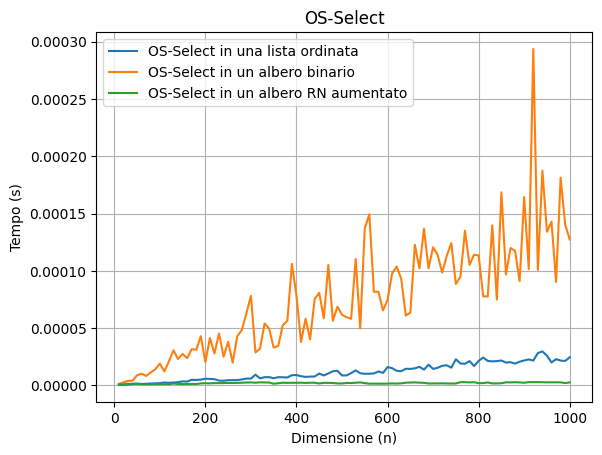
\includegraphics[width=\linewidth/2]{plots/small/os-select-s} }}
	\subfloat[Tempi relativi (interi)]{{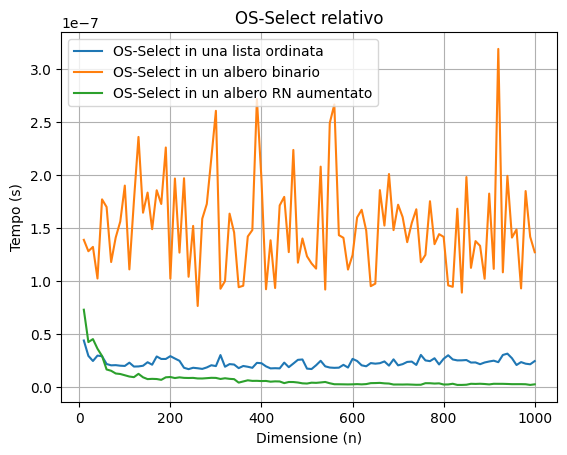
\includegraphics[width=\linewidth/2-1em]{plots/small/os-select-s-rel} }}
    \newline
    \subfloat[Tempi assoluti (float)]{{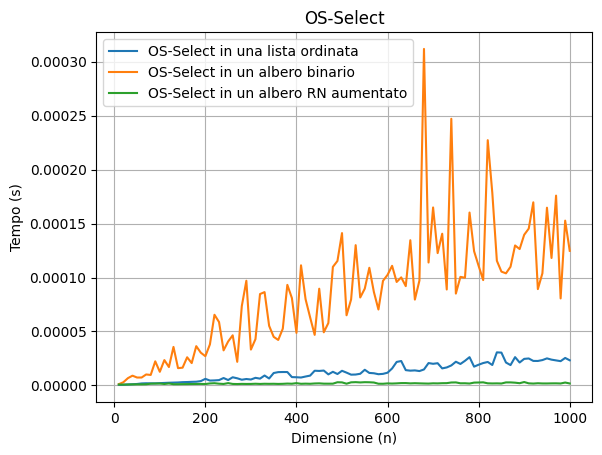
\includegraphics[width=\linewidth/2]{plots/small/os-select-s-float} }}
	\subfloat[Tempi relativi (float)]{{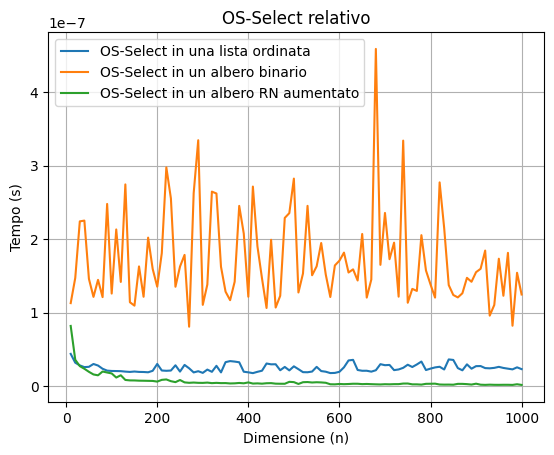
\includegraphics[width=\linewidth/2-1.25em]{plots/small/os-select-s-float-rel} }}
	\caption{Tempi di OS-Select}
	\label{fig:os-select-s}
\end{figure}
\newpage

Come possiamo vedere in \hyperref[fig:os-select-s]{figura 4}, l'operazione di \textit{OS-Select} è molto efficiente per gli alberi rosso-neri aumentati; questo risultato è coerente con la spiegazione teorica fornita nel primo capitolo.

Osserviamo però che non vale lo stesso per gli alberi binari, infatti, su insiemi di dimensioni ridotte sono molto meno efficienti di una lista ordinata; questo è dovuto alla maggiore astrazione che essi offrono, che però non è direttamente utile al calcolo delle statistiche d'ordine dinamiche su un insieme ristretto di valori.

Per strutture con meno di 50 elementi circa, vediamo dai grafici relativi che potrebbe essere conveniente usare una lista ordinata al posto di aggiungere più complessità con un albero rosso nero aumentato.

Semplificando i risultati successivi, possiamo osservare che per insiemi di dimensioni da circa 50 a 1000, popolati con interi o float, le tre strutture dati eseguono \textit{OS-Select} come segue, dalla più veloce alla più lenta:

\begin{enumerate}
    \item \textbf{albero rosso nero aumentato} con media di circa \(0.002\:ms\)
    \item \textbf{lista ordinata} con media di circa \(0.015\:ms\)
    \item \textbf{albero binario} con media di circa \(0.1\:ms\)
\end{enumerate}

Questo trend è ovviamente confermato dai grafici con tempi relativi e anche dai grafici per i dati a virgola mobile, dove viene riscontrato un piccolo aumento dei tempi medi per le tre strutture dati. La differenza più interessante tra i test con interi e quelli con float è quella dell'aumento considerevole della variabilità dei test rispetto alla mediana (osservabile dalle tabelle), rendendo il tempo di esecuzione delle operazioni più difficile da predire.
\newline
\newline
\textit{Riferimenti alle tabelle}: \hyperref[label:lista-ordinata-s-os-select]{OS-Select in una lista ordinata (int)}, \hyperref[label:lista-ordinata-s-float-os-select]{OS-Select in una lista ordinata (float)}, \hyperref[label:abr-s-os-select]{OS-Select in un ABR (int)}, \hyperref[label:abr-s-float-os-select]{OS-Select in un ABR (float)}, \hyperref[label:rn-aumentato-s-os-select]{OS-Select in un albero RN aumentato (int)}, \hyperref[label:rn-aumentato-s-float-os-select]{OS-Select in un albero RN aumentato (float)}.

\begin{figure}[H]
	\subfloat[Tempi assoluti (interi)]{{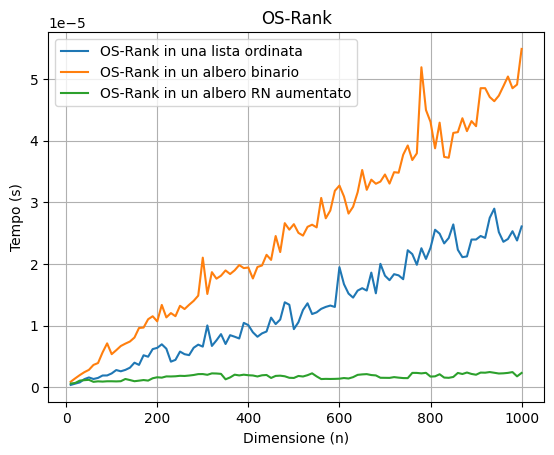
\includegraphics[width=\linewidth/2]{plots/small/os-rank-s} }}
	\subfloat[Tempi relativi (interi)]{{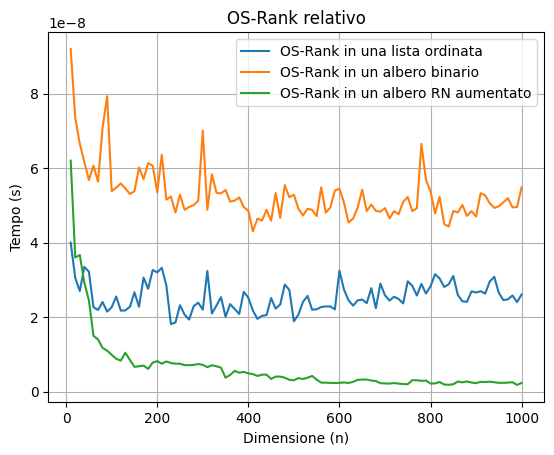
\includegraphics[width=\linewidth/2-0.1em]{plots/small/os-rank-s-rel} }}
    \newline
    \subfloat[Tempi assoluti (float)]{{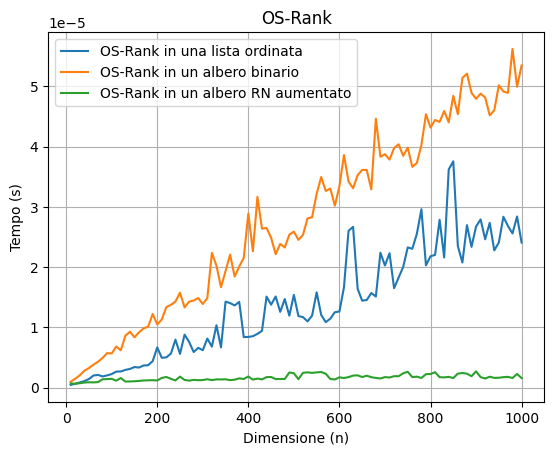
\includegraphics[width=\linewidth/2]{plots/small/os-rank-s-float} }}
	\subfloat[Tempi relativi (float)]{{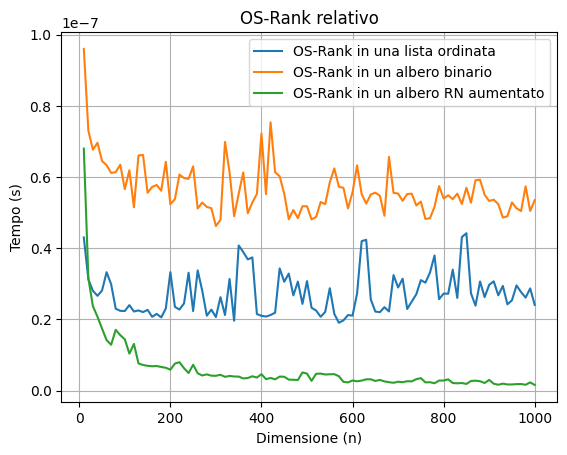
\includegraphics[width=\linewidth/2+0.25em]{plots/small/os-rank-s-float-rel} }}
	\caption{Tempi di OS-Rank}
	\label{fig:os-rank-s}
\end{figure}

Le stesse conclusioni sono valide in linea generale anche per \textit{OS-Rank} come osserviamo in \hyperref[fig:os-rank-s]{figura 5}, l'unica cosa significante è che i tempi dell'\textbf{albero binario} migliorano notevolmente, infatti abbiamo che la media dei risultati si riduce fino a circa \(0.025\:ms\), rimanendo comunque meno efficiente di una lista ordinata.
\newline
\newline
\textit{Riferimenti alle tabelle}: \hyperref[label:lista-ordinata-s-os-rank]{OS-Rank in una lista ordinata (int)}, \hyperref[label:lista-ordinata-s-float-os-rank]{OS-Rank in una lista ordinata (float)}, \hyperref[label:abr-s-os-rank]{OS-Rank in un ABR (int)}, \hyperref[label:abr-s-float-os-rank]{OS-Rank in un ABR (float)}, \hyperref[label:rn-aumentato-s-os-rank]{OS-Rank in un albero RN aumentato (int)}, \hyperref[label:rn-aumentato-s-float-os-rank]{OS-Rank in un albero RN aumentato (float)}.
\newline
\newline
\textit{Riferimenti ai grafici singoli}: \hyperref[label:lista-ordinata-s]{Lista ordinata (int)}, \hyperref[label:lista-ordinata-s-float]{Lista ordinata (float)}, \hyperref[label:abr-s]{ABR (int)}, \hyperref[label:abr-s-float]{ABR (float)}, \hyperref[label:rn-aumentato-s]{Albero RN aumentato (int)}, \hyperref[label:rn-aumentato-s-float]{Albero RN aumentato (float)}.

\newpage
\subsection{Dimensioni medie}

\begin{figure}[H]
	\subfloat[Tempi assoluti (interi)]{{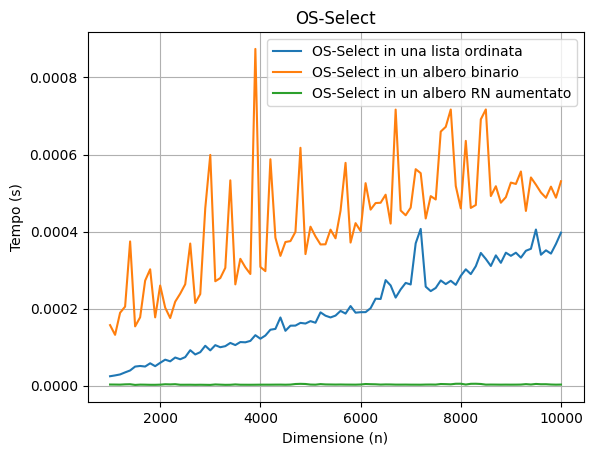
\includegraphics[width=\linewidth/2]{plots/medium/os-select-m} }}
	\subfloat[Tempi relativi (interi)]{{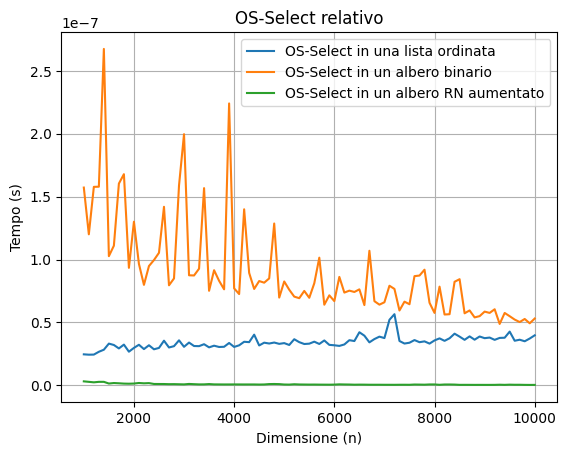
\includegraphics[width=\linewidth/2-0.75em]{plots/medium/os-select-m-rel} }}
    \newline
    \subfloat[Tempi assoluti (float)]{{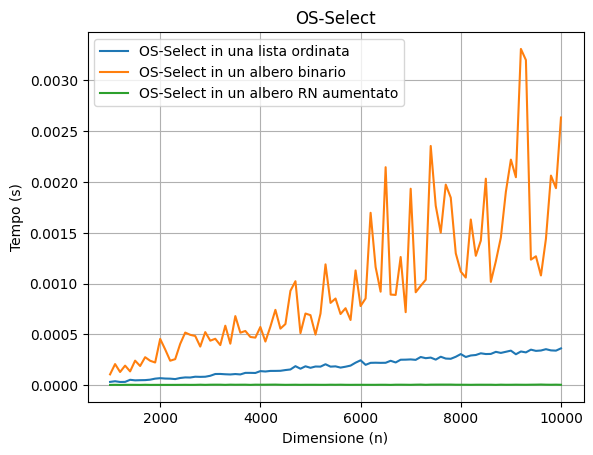
\includegraphics[width=\linewidth/2]{plots/medium/os-select-m-float} }}
	\subfloat[Tempi relativi (float)]{{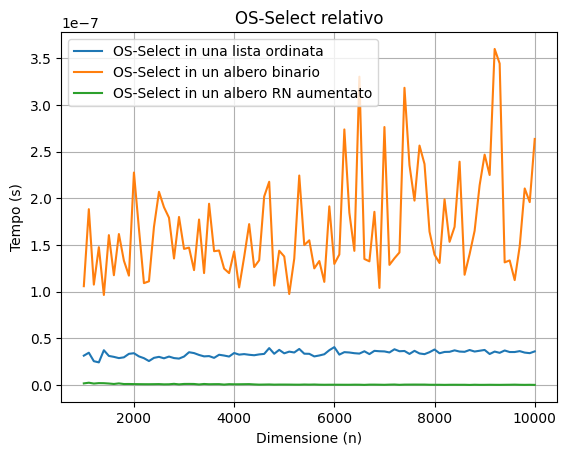
\includegraphics[width=\linewidth/2-0.75em]{plots/medium/os-select-m-float-rel} }}
	\caption{Tempi di OS-Select}
	\label{fig:os-select-m}
\end{figure}

Per le strutture da dimensione 1000 a 10000 vediamo dalla \hyperref[fig:os-select-m]{figura 6} che l'andamento delle prestazioni di \textit{OS-Select} è analogo, notiamo però nel grafico dei tempi relativi per gli interi che la complessità dell'albero binario si avvicina sempre di più a quella della lista ordinata all'aumentare delle dimensioni. I risultati approssimati sono i seguenti:

\begin{enumerate}
    \item \textbf{albero rosso nero aumentato} con media di circa \(0.003\:ms\)
    \item \textbf{lista ordinata} con media di circa \(0.25\:ms\)
    \item \textbf{albero binario} con media di circa \(0.4\:ms\)
\end{enumerate}

Per i dati a virgola mobile non vediamo bene questo andamento, però la differenza relativa tra le prestazioni dell'albero binario e quelle della lista ordinata è inferiore a quanto osservato per le strutture di dimensioni ridotte. 
\newline
\textit{Riferimenti alle tabelle}: \hyperref[label:lista-ordinata-m-os-select]{OS-Select in una lista ordinata (int)}, \hyperref[label:lista-ordinata-m-float-os-select]{OS-Select in una lista ordinata (float)}, \hyperref[label:abr-m-os-select]{OS-Select in un ABR (int)}, \hyperref[label:abr-m-float-os-select]{OS-Select in un ABR (float)}, \hyperref[label:rn-aumentato-m-os-select]{OS-Select in un albero RN aumentato (int)}, \hyperref[label:rn-aumentato-m-float-os-select]{OS-Select in un albero RN aumentato (float)}.

\begin{figure}[H]
	\subfloat[Tempi assoluti (interi)]{{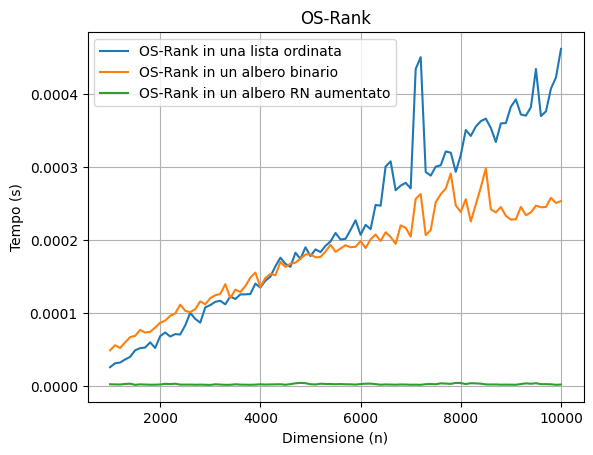
\includegraphics[width=\linewidth/2]{plots/medium/os-rank-m} }}
	\subfloat[Tempi relativi (interi)]{{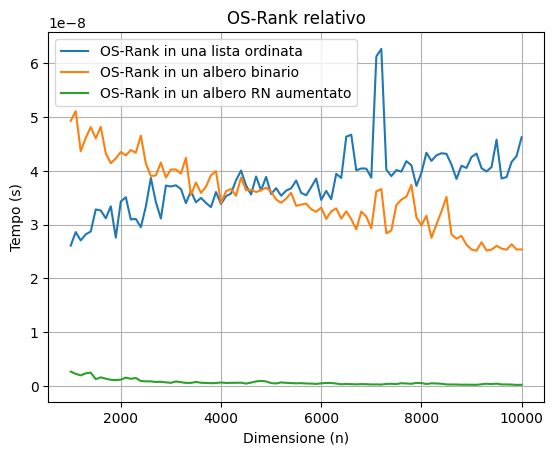
\includegraphics[width=\linewidth/2-1em]{plots/medium/os-rank-m-rel} }}
    \newline
    \subfloat[Tempi assoluti (float)]{{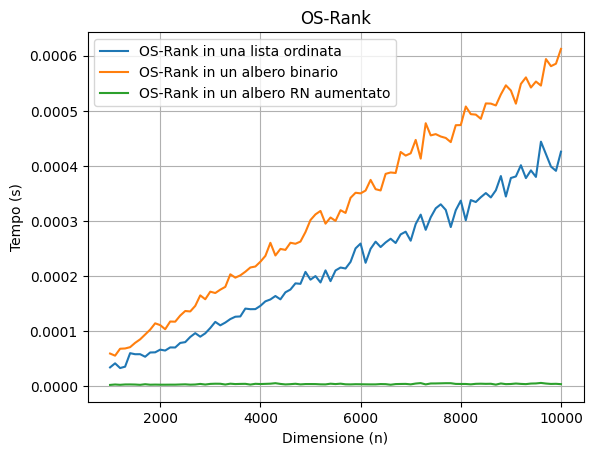
\includegraphics[width=\linewidth/2]{plots/medium/os-rank-m-float} }}
	\subfloat[Tempi relativi (float)]{{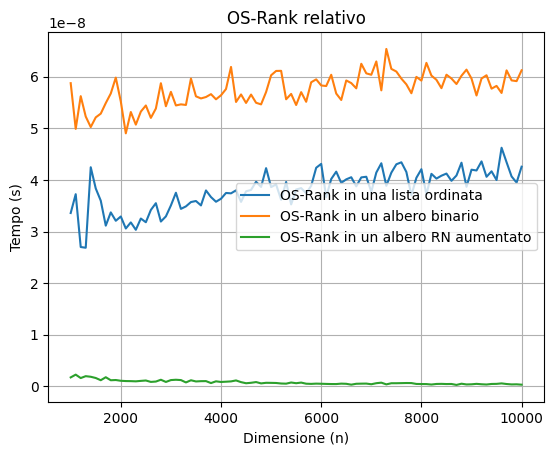
\includegraphics[width=\linewidth/2-1em]{plots/medium/os-rank-m-float-rel} }}
	\caption{Tempi di OS-Rank}
	\label{fig:os-rank-m}
\end{figure}

Vediamo dalla \hyperref[fig:os-rank-m]{figura 7} che la curva dei tempi di \textit{OS-Rank} per un albero binario interseca quella dei tempi per una lista ordinata intorno ai 5000 elementi, questo andamento è anche confermato dal grafico degli andamenti relativi. Le medie approssimative per \textit{OS-Rank} sono analoghe a quelle di OS-Select, tranne l'\textbf{albero binario} che ha media di circa \(0.2\:ms\), superando quindi la lista ordinata su questa operazione.

Non vale lo stesso per i dati a virgola mobile, infatti gli alberi binari sono comunque meno performanti su \textit{OS-Rank} rispetto alle liste ordinate; l'andamento delle due curve dei tempi relativi è oltretutto parallelo con una differenza di circa \(0.2\:ms\) in tempo assoluto.
\newline
\textit{Riferimenti alle tabelle}: \hyperref[label:lista-ordinata-m-os-rank]{OS-Rank in una lista ordinata (int)}, \hyperref[label:lista-ordinata-m-float-os-rank]{OS-Rank in una lista ordinata (float)}, \hyperref[label:abr-m-os-rank]{OS-Rank in un ABR (int)}, \hyperref[label:abr-m-float-os-rank]{OS-Rank in un ABR (float)}, \hyperref[label:rn-aumentato-m-os-rank]{OS-Rank in un albero RN aumentato (int)}, \hyperref[label:rn-aumentato-m-float-os-rank]{OS-Rank in un albero RN aumentato (float)}.
\newline
\newline
\textit{Riferimenti ai grafici singoli}: \hyperref[label:lista-ordinata-m]{Lista ordinata (int)}, \hyperref[label:lista-ordinata-m-float]{Lista ordinata (float)}, \hyperref[label:abr-m]{ABR (int)}, \hyperref[label:abr-m-float]{ABR (float)}, \hyperref[label:rn-aumentato-m]{Albero RN aumentato (int)}, \hyperref[label:rn-aumentato-m-float]{Albero RN aumentato (float)}.

\subsection{Dimensioni elevate}

\begin{figure}[H]
	\subfloat[Tempi assoluti (interi)]{{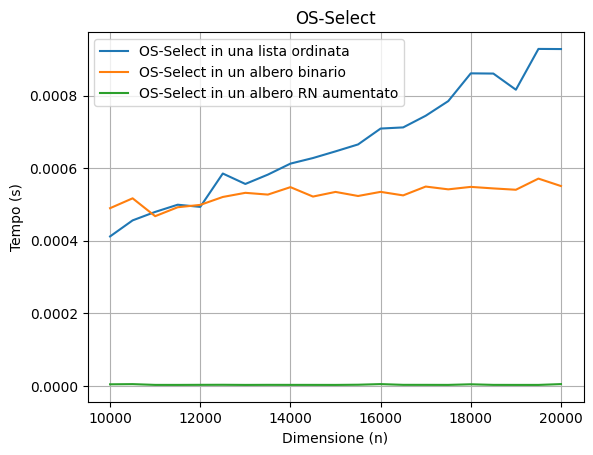
\includegraphics[width=\linewidth/2]{plots/large/os-select-l} }}
	\subfloat[Tempi relativi (interi)]{{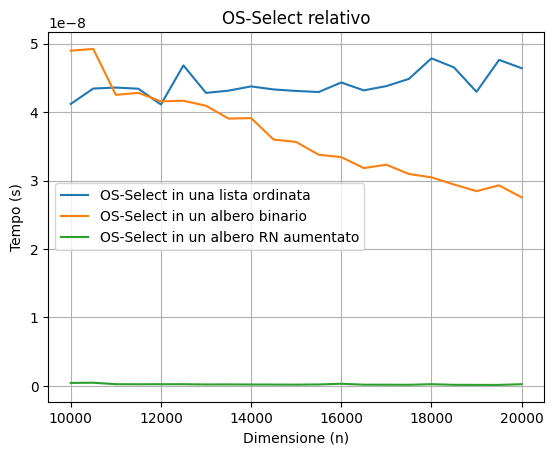
\includegraphics[width=\linewidth/2-1.25em]{plots/large/os-select-l-rel} }}
    \newline
    \subfloat[Tempi assoluti (float)]{{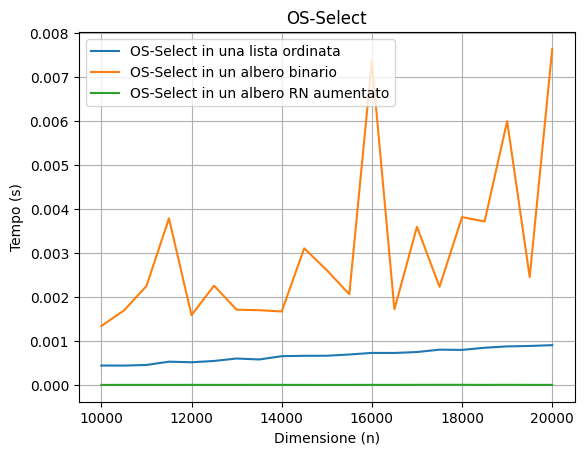
\includegraphics[width=\linewidth/2]{plots/large/os-select-l-float} }}
	\subfloat[Tempi relativi (float)]{{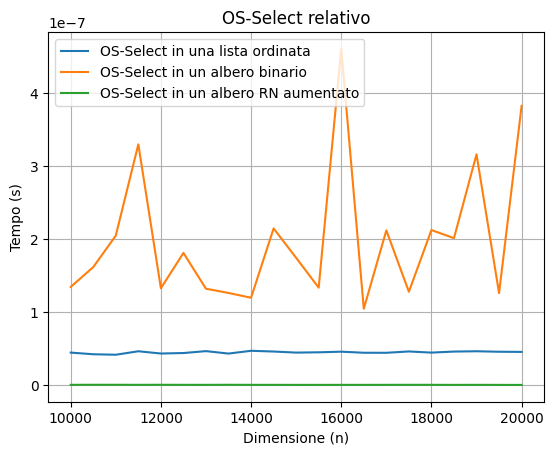
\includegraphics[width=\linewidth/2-1em]{plots/large/os-select-l-float-rel} }}
	\caption{Tempi di OS-Select}
	\label{fig:os-select-l}
\end{figure}

Finalmente per dimensioni superiori circa ai 12000 elementi vediamo che, per l'operazione di \textit{OS-Select} su dati interi, l'albero binario è più efficiente rispetto alla lista ordinata. Questo risultato è in linea con la discussione teorica condotta a all'inizio della relazione. Osserviamo oltretutto dal grafico dei tempi relativi per dati interi in \hyperref[fig:os-select-l]{figura 8} che la curva dell'albero binario scende rapidamente, mentre quella della lista ordinata rimane quasi costante. 

Riassumendo i risultati abbiamo che una operazione di \textit{OS-Select} impiega:
\begin{enumerate}
    \item \textbf{albero rosso nero aumentato} circa \(0.0035\:ms\)
    \item \textbf{albero binario} circa \(0.53\:ms\)
    \item \textbf{lista ordinata} circa \(0.7\:ms\)
\end{enumerate}

Per dati a virgola mobile anche in questo caso non valgono le stesse considerazioni, infatti rimane comunque più performante la \textbf{lista ordinata}. Supponiamo comunque che a dimensioni ancora più elevate riscontreremo lo stesso risultato degli interi, trovando un punto in cui le due curve si intersecano e i tempi dell'albero binario sono migliori di quelli della lista ordinata da quella dimensione in poi.
\newline
\newline
\textit{Riferimenti alle tabelle}: \hyperref[label:lista-ordinata-l-os-select]{OS-Select in una lista ordinata (int)}, \hyperref[label:lista-ordinata-l-float-os-select]{OS-Select in una lista ordinata (float)}, \hyperref[label:abr-l-os-select]{OS-Select in un ABR (int)}, \hyperref[label:abr-l-float-os-select]{OS-Select in un ABR (float)}, \hyperref[label:rn-aumentato-l-os-select]{OS-Select in un albero RN aumentato (int)}, \hyperref[label:rn-aumentato-l-float-os-select]{OS-Select in un albero RN aumentato (float)}.

\begin{figure}[H]
	\subfloat[Tempi assoluti (interi)]{{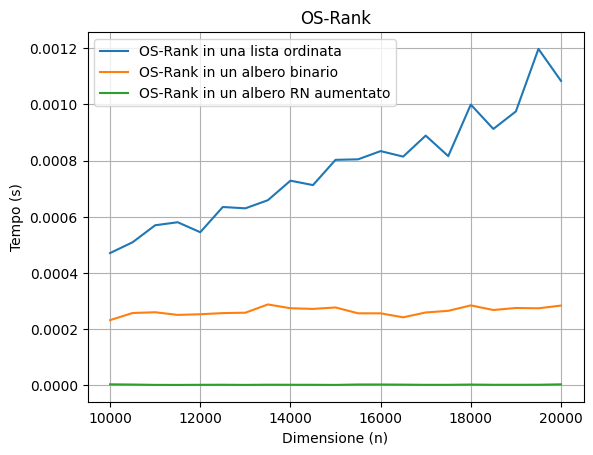
\includegraphics[width=\linewidth/2]{plots/large/os-rank-l} }}
	\subfloat[Tempi relativi (interi)]{{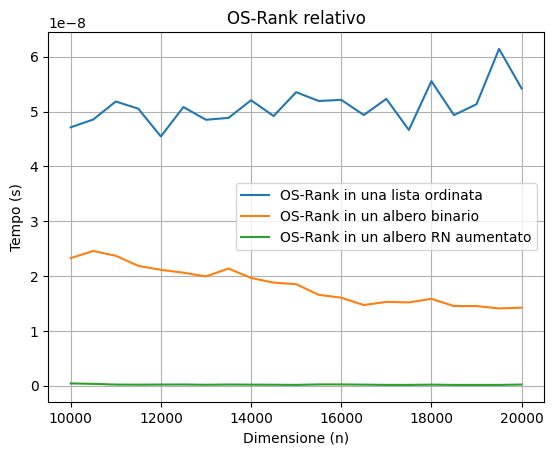
\includegraphics[width=\linewidth/2-1.1em]{plots/large/os-rank-l-rel} }}
    \newline
    \subfloat[Tempi assoluti (float)]{{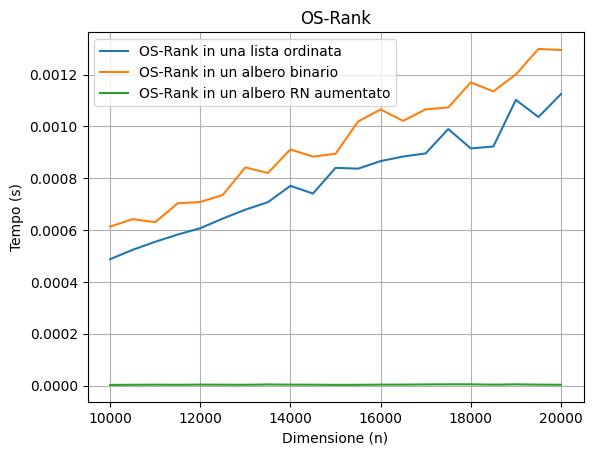
\includegraphics[width=\linewidth/2]{plots/large/os-rank-l-float} }}
	\subfloat[Tempi relativi (float)]{{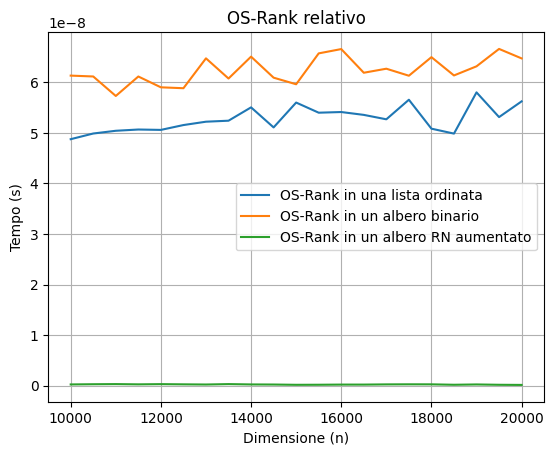
\includegraphics[width=\linewidth/2-1.1em]{plots/large/os-rank-l-float-rel} }}
	\caption{Tempi di OS-Rank}
	\label{fig:os-rank-l}
\end{figure}

In \hyperref[fig:os-rank-l]{figura 9} osserviamo che l'andamento di \textit{OS-Rank} per un albero binario è confermato, infatti la sua curva dei tempi relativi continua a decrescere con l'aumentare della dimensione. Al contrario i tempi per la lista ordinata peggiorano leggermente, infatti avremo:

\begin{enumerate}
    \item \textbf{albero binario} circa \(0.25\:ms\)
    \item \textbf{lista ordinata} circa \(0.8\:ms\)
\end{enumerate}

Per i dati a virgola mobile, la \textbf{lista ordinata} continua comunque ad essere più efficiente degli alberi binari ma la differenza tra le curve dei tempi relativi si assottiglia a circa \(0.1\:ms\) in tempo assoluto. Abbiamo quindi un miglioramento del 50\% rispetto a strutture con dimensione media, supponendo quindi che a dimensioni più elevate di 20000 ci sia un punto di intersezione dove l'andamento dei tempi per l'albero binario si inverta rispetto a quello della lista ordinata per l'operazione di \textit{OS-Rank}. 
\newline
\newline
\textit{Riferimenti alle tabelle}: \hyperref[label:lista-ordinata-l-os-rank]{OS-Rank in una lista ordinata (int)}, \hyperref[label:lista-ordinata-l-float-os-rank]{OS-Rank in una lista ordinata (float)}, \hyperref[label:abr-l-os-rank]{OS-Rank in un ABR (int)}, \hyperref[label:abr-l-float-os-rank]{OS-Rank in un ABR (float)}, \hyperref[label:rn-aumentato-l-os-rank]{OS-Rank in un albero RN aumentato (int)}, \hyperref[label:rn-aumentato-l-float-os-rank]{OS-Rank in un albero RN aumentato (float)}.
\newline
\newline
\textit{Riferimenti ai grafici singoli}: \hyperref[label:lista-ordinata-l]{Lista ordinata (int)}, \hyperref[label:lista-ordinata-l-float]{Lista ordinata (float)}, \hyperref[label:abr-l]{ABR (int)}, \hyperref[label:abr-l-float]{ABR (float)}, \hyperref[label:rn-aumentato-l]{Albero RN aumentato (int)}, \hyperref[label:rn-aumentato-l-float]{Albero RN aumentato (float)}.

\newpage
\section{Conclusioni}

Abbiamo esaminato le prestazioni di \textit{OS-Select} e \textit{OS-Rank} per le tre strutture (liste ordinate, alberi binari e alberi rosso-neri aumentati) in base alle dimensioni dei dati, distinguendo tra dimensioni ridotte, dimensioni piccole, medie ed elevate e considerando sia dati interi che dati a virgola mobile. Ecco le conclusioni principali derivate dai nostri risultati:

\begin{itemize}
\item \textbf{Dimensioni piccole} (meno di 50 elementi): le liste ordinate dimostrano di essere la scelta più efficiente. La loro semplicità e la bassa complessità li rendono ideali per piccoli insiemi di dati, superando sia gli alberi binari che gli alberi rosso-neri aumentati in termini di prestazioni.

\item \textbf{Dimensioni ridotte} (circa 50-1000 elementi): gli alberi rosso-neri aumentati sono la scelta più efficiente, seguiti dalle liste ordinate. Gli alberi binari sono meno efficienti in questo contesto a causa della maggiore astrazione che offrono, che non è direttamente utile per il calcolo delle statistiche d'ordine su insiemi ridotti.

\item \textbf{Dimensioni medie} (circa 1000-12000 elementi): gli alberi rosso-neri aumentati rimangono la scelta più efficiente, seguiti dalle liste ordinate. Tuttavia, gli alberi binari diventano progressivamente più efficienti, avvicinandosi alle prestazioni delle liste ordinate al crescere delle dimensioni.

\item \textbf{Dimensioni elevate} (circa 12000-20000 elementi): gli alberi binari superano le liste ordinate in termini di prestazioni per \textit{OS-Select} e \textit{OS-Rank}, su valori interi. Questo risultato è in linea con le previsioni teoriche. Per dati a virgola mobile, le liste ordinate rimangono comunque più efficienti, anche se la differenza si riduce. Possiamo supporre che a dimensioni ancora più elevate il risultato per dati a virgola mobile sia simile a quello dei dati interi. 
\end{itemize}

Gli alberi rosso-neri aumentati sono una scelta efficace per dimensioni ridotte, medie e elevate, mentre gli alberi binari diventano vantaggiosi rispetto alle liste ordinate per insiemi di dimensioni elevate con dati interi. Per i dati a virgola mobile sono più affidabili le liste ordinate che gli alberi binari in tutte le circostanze osservate.
In generale, la scelta della struttura dati dovrebbe essere guidata dalle esigenze specifiche dell'applicazione, tenendo anche conto delle prestazioni e della complessità di gestione delle diverse strutture (inserimenti, cancellazioni, etc), senza limitarsi alle due operazioni analizzate in questa relazione.

\newpage
\section{Appendice - Grafici e tabelle delle misurazioni}

Tutte le misurazioni effettuate sono disponibili nella \anchor{repository Github}{https://github.com/albbus-stack/lab-alg} in formato \verb|.csv| e anche in formato tabulare in \TeX\, oltre a molti altri grafici per le singole strutture non mostrati esplicitamente in questa relazione. Le tabelle in formato \verb|.csv| sono comodamente consultabili tramite l'interfaccia utente di Github e sono riusabili per qualsiasi altro test, quelle in \TeX\ sono rese disponibili per essere inserite facilmente in altri documenti.

\subsection{Dimensioni ridotte}

\anchor{Grafico lista ordinata (int)}{https://github.com/albbus-stack/lab-alg/blob/main/latex/images/plots/small/lista-ordinata-s.png} \label{label:lista-ordinata-s}
\newline
\anchor{Grafico lista ordinata (float)}{https://github.com/albbus-stack/lab-alg/blob/main/latex/images/plots/small/lista-ordinata-s-float.png} \label{label:lista-ordinata-s-float}
\newline
\anchor{Grafico ABR (int)}{https://github.com/albbus-stack/lab-alg/blob/main/latex/images/plots/small/abr-s.png} \label{label:abr-s}
\newline
\anchor{Grafico ABR (float)}{https://github.com/albbus-stack/lab-alg/blob/main/latex/images/plots/small/abr-s-float.png} \label{label:abr-s-float}
\newline
\anchor{Grafico albero RN aumentato (int)}{https://github.com/albbus-stack/lab-alg/blob/main/latex/images/plots/small/rn-aumentato-s.png} \label{label:rn-aumentato-s}
\newline
\anchor{Grafico albero RN aumentato (float)}{https://github.com/albbus-stack/lab-alg/blob/main/latex/images/plots/small/rn-aumentato-s-float.png} \label{label:rn-aumentato-s-float}

\newpage

\noindent
\anchor{Tabella OS-Select in una lista ordinata (int)}{https://github.com/albbus-stack/lab-alg/blob/main/latex/small-tables/tabelle-lista-ordinata-s-os-select.csv} \label{label:lista-ordinata-s-os-select}
\newline
\anchor{Tabella OS-Select in una lista ordinata (float)}{https://github.com/albbus-stack/lab-alg/blob/main/latex/small-tables/tabelle-lista-ordinata-s-float-os-select.csv} \label{label:lista-ordinata-s-float-os-select}
\newline
\anchor{Tabella OS-Select in un ABR (int)}{https://github.com/albbus-stack/lab-alg/blob/main/latex/small-tables/tabelle-abr-s-os-select.csv} \label{label:abr-s-os-select}
\newline
\anchor{Tabella OS-Select in un ABR (float)}{https://github.com/albbus-stack/lab-alg/blob/main/latex/small-tables/tabelle-abr-s-float-os-select.csv} \label{label:abr-s-float-os-select}
\newline
\anchor{Tabella OS-Select in un albero RN aumentato (int)}{https://github.com/albbus-stack/lab-alg/blob/main/latex/small-tables/tabelle-rn-aumentato-s-os-select.csv} \label{label:rn-aumentato-s-os-select}
\newline
\anchor{Tabella OS-Select in un albero RN aumentato (float)}{https://github.com/albbus-stack/lab-alg/blob/main/latex/small-tables/tabelle-rn-aumentato-s-float-os-select.csv} \label{label:rn-aumentato-s-float-os-select}

\newpage

\noindent
\anchor{Tabella OS-Rank in una lista ordinata (int)}{https://github.com/albbus-stack/lab-alg/blob/main/latex/small-tables/tabelle-lista-ordinata-s-os-rank.csv} \label{label:lista-ordinata-s-os-rank}
\newline
\anchor{Tabella OS-Rank in una lista ordinata (float)}{https://github.com/albbus-stack/lab-alg/blob/main/latex/small-tables/tabelle-lista-ordinata-s-float-os-rank.csv} \label{label:lista-ordinata-s-float-os-rank}
\newline
\anchor{Tabella OS-Rank in un ABR (int)}{https://github.com/albbus-stack/lab-alg/blob/main/latex/small-tables/tabelle-abr-s-os-rank.csv} \label{label:abr-s-os-rank}
\newline
\anchor{Tabella OS-Rank in un ABR (float)}{https://github.com/albbus-stack/lab-alg/blob/main/latex/small-tables/tabelle-abr-s-float-os-rank.csv} \label{label:abr-s-float-os-rank}
\newline
\anchor{Tabella OS-Rank in un albero RN aumentato (int)}{https://github.com/albbus-stack/lab-alg/blob/main/latex/small-tables/tabelle-rn-aumentato-s-os-rank.csv} \label{label:rn-aumentato-s-os-rank}
\newline
\anchor{Tabella OS-Rank in un albero RN aumentato (float)}{https://github.com/albbus-stack/lab-alg/blob/main/latex/small-tables/tabelle-rn-aumentato-s-float-os-rank.csv} \label{label:rn-aumentato-s-float-os-rank}

\newpage
\subsection{Dimensioni medie}

\anchor{Grafico lista ordinata (int)}{https://github.com/albbus-stack/lab-alg/blob/main/latex/images/plots/small/lista-ordinata-m.png} \label{label:lista-ordinata-m}
\newline
\anchor{Grafico lista ordinata (float)}{https://github.com/albbus-stack/lab-alg/blob/main/latex/images/plots/small/lista-ordinata-m-float.png} \label{label:lista-ordinata-m-float}
\newline
\anchor{Grafico ABR (int)}{https://github.com/albbus-stack/lab-alg/blob/main/latex/images/plots/small/abr-m.png} \label{label:abr-m}
\newline
\anchor{Grafico ABR (float)}{https://github.com/albbus-stack/lab-alg/blob/main/latex/images/plots/small/abr-m-float.png} \label{label:abr-m-float}
\newline
\anchor{Grafico albero RN aumentato (int)}{https://github.com/albbus-stack/lab-alg/blob/main/latex/images/plots/small/rn-aumentato-m.png} \label{label:rn-aumentato-m}
\newline
\anchor{Grafico albero RN aumentato (float)}{https://github.com/albbus-stack/lab-alg/blob/main/latex/images/plots/small/rn-aumentato-m-float.png} \label{label:rn-aumentato-m-float}

\newpage

\noindent
\anchor{Tabella OS-Select in una lista ordinata (int)}{https://github.com/albbus-stack/lab-alg/blob/main/latex/small-tables/tabelle-lista-ordinata-m-os-select.csv} \label{label:lista-ordinata-m-os-select}
\newline
\anchor{Tabella OS-Select in una lista ordinata (float)}{https://github.com/albbus-stack/lab-alg/blob/main/latex/small-tables/tabelle-lista-ordinata-m-float-os-select.csv} \label{label:lista-ordinata-m-float-os-select}
\newline
\anchor{Tabella OS-Select in un ABR (int)}{https://github.com/albbus-stack/lab-alg/blob/main/latex/small-tables/tabelle-abr-m-os-select.csv} \label{label:abr-m-os-select}
\newline
\anchor{Tabella OS-Select in un ABR (float)}{https://github.com/albbus-stack/lab-alg/blob/main/latex/small-tables/tabelle-abr-m-float-os-select.csv} \label{label:abr-m-float-os-select}
\newline
\anchor{Tabella OS-Select in un albero RN aumentato (int)}{https://github.com/albbus-stack/lab-alg/blob/main/latex/small-tables/tabelle-rn-aumentato-m-os-select.csv} \label{label:rn-aumentato-m-os-select}
\newline
\anchor{Tabella OS-Select in un albero RN aumentato (float)}{https://github.com/albbus-stack/lab-alg/blob/main/latex/small-tables/tabelle-rn-aumentato-m-float-os-select.csv} \label{label:rn-aumentato-m-float-os-select}

\newpage

\noindent
\anchor{Tabella OS-Rank in una lista ordinata (int)}{https://github.com/albbus-stack/lab-alg/blob/main/latex/small-tables/tabelle-lista-ordinata-m-os-rank.csv} \label{label:lista-ordinata-m-os-rank}
\newline
\anchor{Tabella OS-Rank in una lista ordinata (float)}{https://github.com/albbus-stack/lab-alg/blob/main/latex/small-tables/tabelle-lista-ordinata-m-float-os-rank.csv} \label{label:lista-ordinata-m-float-os-rank}
\newline
\anchor{Tabella OS-Rank in un ABR (int)}{https://github.com/albbus-stack/lab-alg/blob/main/latex/small-tables/tabelle-abr-m-os-rank.csv} \label{label:abr-m-os-rank}
\newline
\anchor{Tabella OS-Rank in un ABR (float)}{https://github.com/albbus-stack/lab-alg/blob/main/latex/small-tables/tabelle-abr-m-float-os-rank.csv} \label{label:abr-m-float-os-rank}
\newline
\anchor{Tabella OS-Rank in un albero RN aumentato (int)}{https://github.com/albbus-stack/lab-alg/blob/main/latex/small-tables/tabelle-rn-aumentato-m-os-rank.csv} \label{label:rn-aumentato-m-os-rank}
\newline
\anchor{Tabella OS-Rank in un albero RN aumentato (float)}{https://github.com/albbus-stack/lab-alg/blob/main/latex/small-tables/tabelle-rn-aumentato-m-float-os-rank.csv} \label{label:rn-aumentato-m-float-os-rank}

\newpage
\subsection{Dimensioni elevate}

\anchor{Grafico lista ordinata (int)}{https://github.com/albbus-stack/lab-alg/blob/main/latex/images/plots/small/lista-ordinata-l.png} \label{label:lista-ordinata-l}
\newline
\anchor{Grafico lista ordinata (float)}{https://github.com/albbus-stack/lab-alg/blob/main/latex/images/plots/small/lista-ordinata-l-float.png} \label{label:lista-ordinata-l-float}
\newline
\anchor{Grafico ABR (int)}{https://github.com/albbus-stack/lab-alg/blob/main/latex/images/plots/small/abr-l.png} \label{label:abr-l}
\newline
\anchor{Grafico ABR (float)}{https://github.com/albbus-stack/lab-alg/blob/main/latex/images/plots/small/abr-l-float.png} \label{label:abr-l-float}
\newline
\anchor{Grafico albero RN aumentato (int)}{https://github.com/albbus-stack/lab-alg/blob/main/latex/images/plots/small/rn-aumentato-l.png} \label{label:rn-aumentato-l}
\newline
\anchor{Grafico albero RN aumentato (float)}{https://github.com/albbus-stack/lab-alg/blob/main/latex/images/plots/small/rn-aumentato-l-float.png} \label{label:rn-aumentato-l-float}

\newpage

\noindent
\anchor{Tabella OS-Select in una lista ordinata (int)}{https://github.com/albbus-stack/lab-alg/blob/main/latex/small-tables/tabelle-lista-ordinata-l-os-select.csv} \label{label:lista-ordinata-l-os-select}
\newline
\anchor{Tabella OS-Select in una lista ordinata (float)}{https://github.com/albbus-stack/lab-alg/blob/main/latex/small-tables/tabelle-lista-ordinata-l-float-os-select.csv} \label{label:lista-ordinata-l-float-os-select}
\newline
\anchor{Tabella OS-Select in un ABR (int)}{https://github.com/albbus-stack/lab-alg/blob/main/latex/small-tables/tabelle-abr-l-os-select.csv} \label{label:abr-l-os-select}
\newline
\anchor{Tabella OS-Select in un ABR (float)}{https://github.com/albbus-stack/lab-alg/blob/main/latex/small-tables/tabelle-abr-l-float-os-select.csv} \label{label:abr-l-float-os-select}
\newline
\anchor{Tabella OS-Select in un albero RN aumentato (int)}{https://github.com/albbus-stack/lab-alg/blob/main/latex/small-tables/tabelle-rn-aumentato-l-os-select.csv} \label{label:rn-aumentato-l-os-select}
\newline
\anchor{Tabella OS-Select in un albero RN aumentato (float)}{https://github.com/albbus-stack/lab-alg/blob/main/latex/small-tables/tabelle-rn-aumentato-l-float-os-select.csv} \label{label:rn-aumentato-l-float-os-select}

\newpage

\noindent
\anchor{Tabella OS-Rank in una lista ordinata (int)}{https://github.com/albbus-stack/lab-alg/blob/main/latex/small-tables/tabelle-lista-ordinata-l-os-rank.csv} \label{label:lista-ordinata-l-os-rank}
\newline
\anchor{Tabella OS-Rank in una lista ordinata (float)}{https://github.com/albbus-stack/lab-alg/blob/main/latex/small-tables/tabelle-lista-ordinata-l-float-os-rank.csv} \label{label:lista-ordinata-l-float-os-rank}
\newline
\anchor{Tabella OS-Rank in un ABR (int)}{https://github.com/albbus-stack/lab-alg/blob/main/latex/small-tables/tabelle-abr-l-os-rank.csv} \label{label:abr-l-os-rank}
\newline
\anchor{Tabella OS-Rank in un ABR (float)}{https://github.com/albbus-stack/lab-alg/blob/main/latex/small-tables/tabelle-abr-l-float-os-rank.csv} \label{label:abr-l-float-os-rank}
\newline
\anchor{Tabella OS-Rank in un albero RN aumentato (int)}{https://github.com/albbus-stack/lab-alg/blob/main/latex/small-tables/tabelle-rn-aumentato-l-os-rank.csv} \label{label:rn-aumentato-l-os-rank}
\newline
\anchor{Tabella OS-Rank in un albero RN aumentato (float)}{https://github.com/albbus-stack/lab-alg/blob/main/latex/small-tables/tabelle-rn-aumentato-l-float-os-rank.csv} \label{label:rn-aumentato-l-float-os-rank}

\end{document}